\documentclass[a4paper, 12pt, twoside, openright, fleqn]{book}

% language settings
\usepackage[italian]{babel}
\usepackage[T1]{fontenc}
\usepackage[utf8]{inputenc}
\usepackage{fancyhdr}
\usepackage{subcaption}
\usepackage[usenames, dvipsnames, table, tikz]{xcolor}
\usepackage{tikz,float,pdfpages,pgfplots,listing, steinmetz}
\usepackage{graphicx,graphics,wrapfig,changepage}

% math package
\usepackage{mathtools,amsthm,environ,cancel,cases}
\usepackage{amsmath, amssymb, dsfont, bm,blkarray}
\graphicspath{{./img/} {./.tmp/} }
% tikz figures
% \usepackage{tikz}
\usetikzlibrary{shapes, arrows, automata,circuits.ee.IEC}
\tikzset{blk/.style={draw, minimum size=0.5cm, text width = 1.8 cm}}
\tikzset{chan/.style={cylinder,shape aspect = 0.2,draw, minimum size=0.5cm, text width = 1.5 cm}}
% add support for url and cross-references in PDF output
\usepackage{url}
\renewcommand{\UrlFont}{\color{black}\small\ttfamily}
\usepackage[colorlinks=true, linkcolor=black, citecolor=black, urlcolor=black]{hyperref}

% support for glossary and acronyms
\usepackage[acronym]{glossaries}
% \newacronym{geraf}{GeRaF}{Geographic Random Forwarding}
% Costumization of theorem style
\newtheoremstyle{theoremdd}% name of the style to be used
  {\topsep}% measure of space to leave above the theorem. E.g.: 3pt
  {\topsep}% measure of space to leave below the theorem. E.g.: 3pt
  {\itshape}% name of font to use in the body of the theorem
  {0pt}% measure of space to indent
  {\bfseries}% name of head font %\color{Mahogany}
  { -- }% punctuation between head and body
  { }% space after theorem head; " " = normal interword space
  {\thmname{#1}\thmnumber{ #2}\thmnote{ (#3)}}

\theoremstyle{theoremdd}
% support for counting
\newtheorem{theorem}{Theorem}[section]
\newtheorem{corollary}{Corollary}[theorem]
\newtheorem{lemma}[theorem]{Lemma}
\newtheorem{definition}{Definition}
\newtheorem{remark}{Remark}
\newtheorem{example}{Example}

% added support for proof parts
\theoremstyle{remark}
\newtheorem{proofpart}{Part}
\renewcommand\theproofpart{\Roman{proofpart}}
\makeatletter
\@addtoreset{proofpart}{theorem}
\makeatother

% specific modification to basic book template of our book document
% \renewcommand{\chaptername}{Section}
% \addto\captionsenglish{\renewcommand{\chaptername}{Section}}

% \renewcommand\qedsymbol{\includegraphics[width=1.5cm]{occhiali}}
%\renewcommand\qedsymbol{$\square$\itshape QED}

%split and equation environment
\NewEnviron{esp}{%
\begin{equation}\begin{split}
  \BODY
\end{split}\end{equation}
}

\NewEnviron{esp*}{%
\begin{equation*}\begin{split}
  \BODY
\end{split}\end{equation*}
}


%------------------------------ define Abstract environment, missing in the 'book' class
\newenvironment{abstract}{\cleardoublepage \null \vfill \begin{center}\bfseries\abstractname \end{center}}{\vfill\null}
\addto\captionsenglish{\renewcommand*\abstractname{Sommario}} % change Abstract title
%------------------------------ active url
\usepackage{url}
%\usepackage{svg}
\usepackage{ifluatex}
\renewcommand{\UrlFont}{\color{black}\small\ttfamily}

% \usepackage[colorlinks=true, linkcolor=black, citecolor=black, urlcolor=black]{hyperref} % active ref

%------------------------------ macros
\newcommand{\sectionname}{Section} % define Section ref
\newcommand{\subsectionname}{Sub-section} % define Sub-section ref
\renewcommand*\arraystretch{1.4} % tables padding
\newcommand{\N}{\mathcal{N}}
\DeclareInputText{176}{°}

% Useful Aliases
\def\beq{\begin{equation}}
\def\eeq{\end{equation}}
\def\bal{\begin{align}}
\def\eal{\end{align}}
\def\prob{\ensuremath\mathbb{P}}
\def\exp{\ensuremath\mathbb{E}}
\def\pois{\mathcal P}
\newcommand{\Hb}{\mathbb{H}}
\newcommand{\Sb}{\mathbb{\Sigma}}
\newcommand{\U}{\mathbb{U}}
\newcommand{\F}{\mathbb{F}}
\newcommand{\V}{\mathbb{V}}
\newcommand{\A}{\mathbb{A}}
\newcommand{\B}{\mathbb{B}}
\newcommand{\C}{\mathbb{C}}
\newcommand{\E}{\mathbb{E}}
\newcommand{\I}{\mathbb{I}}
\newcommand{\Y}{\mathbb{Y}}
%\newcommand{\N}{\mathbb{N}}
\newcommand{\W}{\mathbb{W}}
\newcommand{\Z}{\mathbb{Z}}
\newcommand{\R}{\mathbb{R}}
\newcommand{\X}{\mathbb{X}}
\renewcommand{\Pr}{\mathbb{P}} %probability
\renewcommand{\P}{\mathcal{P}} % distribution
\newcommand{\Q}{\mathbb{Q}}
\newcommand{\D}{\mathbb{D}}
\newcommand{\Rm}{\mathbb{R^{-1}}}
\newcommand{\J}{\mathbb{J}}
\newcommand*{\Chi}{\mbox{\Large $\chi$}}% big chi
\newcommand{\Fig}[1]{Fig.~\ref{#1}}
\newcommand{\eq}[1]{(\ref{#1})}
\newcommand{\Tab}[1]{Tab.~\ref{#1}}
\newcommand{\Sec}[1]{Sec.~\ref{#1}}
\newcommand{\indep}{\mathrel{\perp\mspace{-10mu}\perp}}
\newcommand{\RN}[1]{ \textup{\uppercase\expandafter{\romannumeral#1}}} 
\newcommand{\curarr}{\rotatebox[origin=c]{180}{$\Lsh$}}
%This is for inserting Roman Numbers (useful for \stackrel in equations so that you don't confuse indicating numbers from equation numbers

\begin{document}
\frontmatter

\begin{titlepage} %------------------------------ TITLE PAGE
\begin{center}

\hspace{0.5cm}

\emph{\Large{TELECOMMUNICATION NETWORKS}} \\
\vspace{1cm}
% \includegraphics[width=9cm]{img/bella.png}\\
\vspace{0.5cm}
{written with foolness by\par}
{\Large Matilde Boschiero\par}
\end{center}

\vfill
\begin{center}
\noindent\makebox[\linewidth]{\rule{\textwidth}{0.4pt}}
\textsc{Academic Year 2017/2018}
\end{center}
\end{titlepage}

\begingroup %------------------------------ CONTENTS
  \makeatletter
  \let\ps@plain\ps@empty
  \makeatother
  \tableofcontents
  \clearpage
\endgroup
\mainmatter
\chapter{Internet}
The Internet is a global system of interconnected computer networks that use the standard \textit{Internet
Protocol Suite (TCP/IP)} to serve several billion users worldwide. We can refer to it as a \textit{Network of Networks}.
\section{Overview}
\begin{itemize}
\item 1961-64: Leonard Kleinrock, a brilliant MIT student, proves that packet switching is very efficient in presence of bursty traffic
\item 1967: Lawrence Roberts $\rightarrow$ \textit{Interface Message Processor (IMP)}: 
\begin{equation}
\begin{cases}
\text{Aim} \rightarrow \text{Interconnect \textbf{heterogeneous host computers through special nodes}}\\
\text{Fundation} \rightarrow \text{Advanced Research Projects Agency (ARPA)}
\end{cases}
\end{equation}
(ARPA) $\in$ Department Of Defense (DoD) of USA $\rightarrow$ dawn of ARPAnet
\item 1969: ARPANET is up and running
\begin{equation}
\begin{cases}
\text{4 nodes}\rightarrow \text{UCLA, UCSB, Stanford Research Inst. (SRI), Utha Univ.}\\
\text{One single protocol} \rightarrow \text{\textit{Network Control Protocol (NCP): RFC 001}} 
\end{cases}
\end{equation}
The first telnet from UCLA to SRI crashes the system$\rightarrow$dawn of the demo effect
\item 1970: ALOHAnet $\rightarrow$ A wireless network to interconnect campuses of Hawaii islands
\item 1970-1980: proliferation of different (\textbf{not interconnected) heterogeneous networks}
\item 1972: Vint Cerf $\&$ Bob Kahn $\rightarrow$ \textit{Gateaways concept}
\begin{definition}{\textbf{Gateway}}
\label{Gateway}

Gateways are special devices (router) used to interconnect heterogeneous networks. They can be Interior (IG) or Exterior (EG) and act as \textbf{universal translator} between heterogeneous networks
\end{definition}
\begin{itemize}
\item Issues: Due to the heterogeneity of the networks we have to manage different packet sizes, interfaces, transmit rates, reliability $\rightarrow$ mess

\end{itemize}
\item A reliable transport protocol, called \textit{Transmission Control Protocol (TCP)}: 
\begin{equation}
\begin{cases}
\bullet \text{ Manage \textbf{e2e communications} over such a heterogeneous mix of Nets.}\\
\bullet \textbf{\text{ TCP shifts the burden of error control recovery from IMP}}\\\text{\textbf{ and to end hosts}}
\end{cases}
\end{equation}
$\Rightarrow$This is the key for the Internet scalability
\item 1977: ARPANET, ALOHANET, Packet Radio network are interconnected as ARPA Internet

$\rightarrow$ Cerf and Kahn proposed to split TCP into TCP (Transmission Control Protocol) $\&$ IP (Internet Protocol), the two most important protocols defined in the suite of protocols TCP
\item 1981: UNIX includes the TCP/IP protocols
\item 1983: ARPANET (with more than 200 nodes) replaces NCP with TCP/IP 
\item National Science Foundation funded CSNET to link computer science departments
across the country and connects to ARPANET through TCP/IP
\item 1983: Birth of the \textit{Domain Name Server (DNS)} system
\item 1990: ARPANET is decommissioned
\item 1994 NFSNET is decommissioned
\textbf{\item 1995: the INTERNET becomes fully commercial}
\item Today, more than 40,000 networks are interconnected by means of TCP/IP
protocols... 40 years back by Cerf and Kahn (ah.. golden ’70!)
\end{itemize}

\section{ISP and NAP}
\begin{definition}{\textbf{Internet Service Provider $\&$ Network Access Point}}
\item $\rhd$ Internet Service Provider 
\item $\rhd$ A Network Access Point is a private institution that provides ISPs interconnection $\rightarrow$ Es: NAP can link National ISPs as TELECOM ITALIA, GARR and FASTWEB but also Local ISPs as UniPD
\end{definition}
\subsection{Inside a ISP}
\begin{itemize}
\item Huge network (company) that collects other smaller ones
\item 2 types of Gateways: special devices to interconnect heterogeneous networks
\begin{equation}
\begin{cases}
IG \rightarrow \text{Internal Gateway}\\
EG \rightarrow \text{Exterior Gateway}
\end{cases}
\end{equation}

\item ISPs are connected in a quasi "hierarchical" manner
\begin{equation}
\begin{cases}
\text{ National ISP} \stackrel{Physical Link}{\longrightarrow} EG \in \text{$\{$Regional ISPs, Local ISPs$\}$}\\
\text{ Regional ISPs} \stackrel{Log + Phy Links}{\longrightarrow} EG \in \text{$\{$ Regional ISPs, Local ISPs$\}$}
\end{cases}
\end{equation}

\item \textbf{Internet is a distributed network in which every ISP interconnects
its backbone to every other ISP}.

\item In Italy several networks, differentiated for services offered and
for geographic coverage, coexist.

\item \textbf{This efficient and effective interconnection between different networks is crucial because it impacts both individual backbones and the global network.}

$\Rightarrow$ MIX: Biggest Italian NAP 
\end{itemize}

\subsection{MIX}
MIX is a point of multiple connection in which the networks of each player (ISP, carrier, content provider, hoster etc…) interconnect themselves to exchange IP traffic (peering) efficiently and with advantageous costs compared to the transit.

$\Rightarrow$ Charateristics:
\begin{equation}
\begin{cases}
\bullet \text{ Handles a vast traffic exchange}\\
\bullet \text{ Promote the development of Internet in Italy}\\
\bullet \text{ Improve the interconnection between different ISPs operating in Italy}\\
\bullet \text{ Is a \textit{point of “multiple
interconnection”}}\\
\bullet \text{ Does not provide IA to public accounts}\\
\bullet \text{ Does not publish content}\\
\bullet \text{ Does not sell web spaces}\\
\bullet \text{ Does not offer web-hosting or web-housing services.}
\end{cases}
\end{equation}
$\Rightarrow$ Customers:
\begin{equation}
\begin{cases}
\bullet \text{ Internet Operators} \rightarrow Peers:\text{agreements with other ISPs connected}\\
\bullet \text{ Carriers} \rightarrow \text{telecom } op_s \text{ that give transit services from and to MIX}\\
\bullet \text{ Operators of root-name servers} \rightarrow \text{super-partes services}\\
\bullet \text{ Operators of Top Level Domain}\\
\end{cases}
\end{equation}

\section{Administration}
\begin{enumerate}
\item Internet Society (ISOC)
\item Internet Architecture Board (IAB)
\begin{enumerate}
\item Internet Engineering Task Force (IETF)
\begin{enumerate}
\item Internet Engineering Steering Group (IESG)\\
\rotatebox[origin=c]{180}{$\Lsh$} Areas $\rightarrow$ Working Groups
\item RFC Editor
\end{enumerate}
\item Internet Research Task Force (IRTF)
\begin{enumerate}
\item Internet Research Steering Group (IRSG)\\
$\rightarrow$ Research Groups
\end{enumerate}
\item Internet Assigned Numbers Authority (IANA)
\begin{enumerate}
\item ICANN
\begin{enumerate}
\item GNSO
\item ASO
\item ACs
\item CCNSO
\item National Telecommunications and Information Administration (NTIA)
\end{enumerate}
\end{enumerate}
\end{enumerate}
\end{enumerate}

\section{Architecture}
\subsection{Structure of a TLC network}
\begin{itemize}
\item Items:
\begin{equation}
\begin{cases}
\bullet \text{ \textbf{Terminal Devices}} \rightarrow \text{PC, phones, screens, speakers storing unit}\\
\bullet \text{ \textbf{Switching Units}: create a communication setup } \\ \rotatebox[origin=c]{180}{$\Lsh$} \text{ Routers: Data Networks} \\ \rotatebox[origin=c]{180}{$\Lsh$} \text{Switches: Telephone Networks}\\
\bullet \text{ \textbf{Links}} \rightarrow \text{Fibre optic, copper, twisted pairs, radio}
\end{cases}
\end{equation}
$\Rightarrow$ Everything is ruled by \textit{Protocols and Interfaces}
$\Rightarrow$ Important items: Hosts (End Systems), Servers, Mobiles, Packet Switches, Modems, Base stations, Satellite links 

\item \textit{\textbf{Access Network = Edge Network}} $\rightarrow$ Provide access to communication services to the hosts\\
$\rotatebox[origin=c]{180}{$\Lsh$}$ \textit{Edge Router = Border Gateway} $\rightarrow$ Belong to both access and transit network \\ $\rotatebox[origin=c]{180}{$\Lsh$}$ May have different topologies
\item \textit{\textbf{Transport Network = Core Network}}\\ $\rotatebox[origin=c]{180}{$\Lsh$}$ Interconnect different Access Networks \\ $\rotatebox[origin=c]{180}{$\Lsh$}$ Transfer \textit{Information Units (IUs)} over long distances\\
$\rotatebox[origin=c]{180}{$\Lsh$}$ May have hierarchical structure \\ $\rotatebox[origin=c]{180}{$\Lsh$}$ \textit{Core Router = Interior Gateways} $\rightarrow$ Belong to the Core Network \textbf{only} 
\item Information transfers: ways of transfer IUs through a network is defined by \textit{Protocols, Multiplexing and Switching}.
\end{itemize}

\subsection{Topologies}
\begin{itemize}
\item Physical topology $\rightarrow$ Graph formed by nodes and physical links

\begin{itemize}
\item Star
\item Mesh
\item Tree
\item Ring
\item Bus
\end{itemize}
\item Logical topology $\rightarrow$ Graph formed by \textit{information flows}
\end{itemize}

\section{Information Transfer}
\begin{definition}{\textbf{Hop}\\}
A hop in a TLC Network is the next node we're referring to reach a specific information transfer. 
\end{definition}

The way of transfer Information Units (IUs) through a Network is defined by:
\begin{equation}
\begin{cases}
\bullet \text{ Protocols}\\
\bullet \text{ Multiplexing}\\
\bullet \text{ Switching}
\end{cases}
\end{equation}

\subsection{Switching}

Switching Nodes $\rightarrow$ Connect multiple communication links \\ $\rotatebox[origin=c]{180}{$\Lsh$}$ Each Switching Node is composed by:
\begin{itemize}
\item \textit{Ingress Ports = Input Ports} $\rightarrow$ Devices that \textbf{receive data} from the connected links $\Rightarrow$ Represented by a \textbf{Queueing Buffer}
\item \textit{Egress Ports = Output Ports} $\rightarrow$ Devices that \textbf{transmit data} on the connected link $\Rightarrow$ Represented by a \textbf{Queueing Buffer}
\item \textit{Switching Logic} $\rightarrow$ Mechanism that makes it possible to transfer an Information Unit (IU) from one input port to an output port 
\end{itemize}

\subsection{Types of Switching}
3 types of Switching:
\begin{enumerate}
\item Circuit Switching
\item Virtual Switching
\item Packet Switching 
\end{enumerate}

\subsection{Circuit Switching}
\begin{equation}
\begin{cases}
\bullet \text{ Using dedicated resources the performances} \\ \text{ are guaranteed but there's a no negligible risk of blocking}\\
\bullet \text{ Circuit-switched networks require dedicated point-to-point}\\ \text{ connections during calls}\\
\end{cases}
\end{equation}

\subparagraph{CS-Networks}
\begin{figure}
\centering
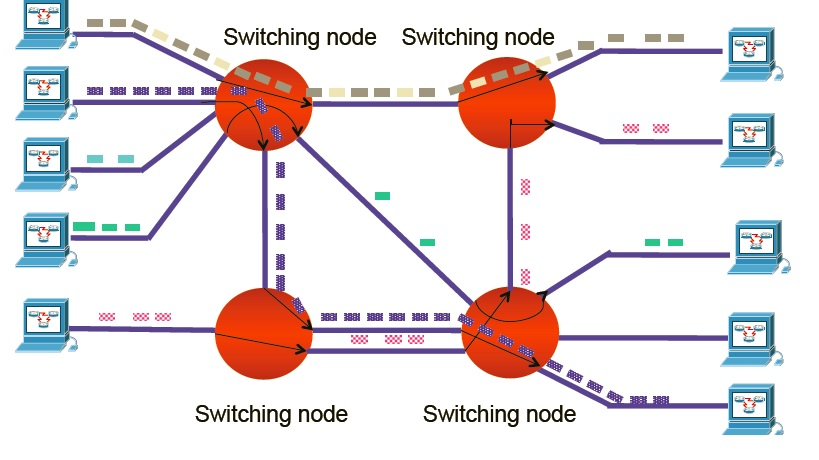
\includegraphics[width=0.8\textwidth]{CS.jpg}
\caption{\label{CS.jpg}Circuit Switching}
\end{figure}

\begin{itemize}
\item Are used for phone calls
\item Reserve a dedicated channel for the entire communication
\item Private Branch EXchange (PBX) system: First hardware for a circuit-switched network 
\item \textsc{Working Operation:} 
\begin{equation}
\begin{cases}
\bullet \text{ Electronic signals pass through several switches before a connec-}\\ \text{ -tion is established}\\
\bullet \text{\textbf{ During a call, no other network traffic can use those}} \\ \text{\textbf{ switches.}}
\end{cases}
\end{equation}
\end{itemize}

\subsection{Virtual Switching}

\subsection{Packet Switching}
\begin{equation}
\begin{cases}
\bullet \text{ Packet-switched networks move data in packets based on the}\\ \text{ destination address in each packet} \\
\bullet \text{ When received, packers are reassembled in the proper sequence} \\ \text{ to make up the original message}\\
\bullet \text{ Shared Resources} \rightarrow \text{Best Effort}
\end{cases}
\end{equation}

It consists in two basic operations:
\begin{equation}
\begin{cases}
\bullet \text{\textit{ \textbf{Routing}}}\\ \rotatebox[origin=c]{180}{$\Lsh$} \text{ Selection of the next hop}\\ \rotatebox[origin=c]{180}{$\Lsh$} \text{ Insertion of the IU in the buffer of the corrisponding output port}\\
\rotatebox[origin=c]{180}{$\Lsh$} \text{ Performed via software to allow for update of routing algorithms}\\
\bullet \text{ \textit{\textbf{Forwarding}}}\\ \rotatebox[origin=c]{180}{$\Lsh$} \text{ Physical transmission of the IU to the next hop}
\\ \rotatebox[origin=c]{180}{$\Lsh$} \text{ Is a \textit{hardware} operation}
\end{cases}
\end{equation}
The fact that the \textbf{forwarding} is a \textit{hardware} operation is due to \textbf{predetermination of the transmission techniques} $\rightarrow$ If a better transmission technique is available you just update the \textit{Network Interface Card (NIC)} of your switch $\rightarrow$ No need to change the routing software.

\subparagraph{PS-Networks}
\begin{figure}
\centering
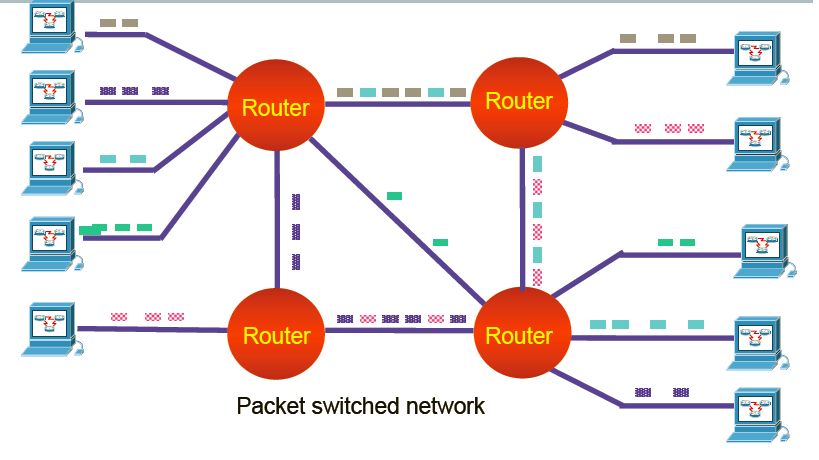
\includegraphics[width=0.8\textwidth]{PS.png}
\caption{\label{PS.png}Packet switching}
\end{figure}
\begin{itemize}
\item Are used to handle data
\item Power Computer Servers
\item \textsc{Working Operation:} 
\begin{equation}
\begin{cases}
\bullet \text{ The message gets broken into small data packets that seek out} \\ \text{ the most efficient route as circuits become available}\\
\bullet \text{ Each packet may go a different route.}\\
\bullet \text{ Its \textbf{header address tells it where to go and describes}} \\ \text{the sequence for reassembly at the destination compute.}\\
\bullet \text{ Packets arrival} \rightarrow \text{Queue of packets} \rightarrow \text{Statistical Multiplexing}
\end{cases}
\end{equation}
\end{itemize}
 
 
\subparagraph{Buffering}
\begin{figure}
\centering
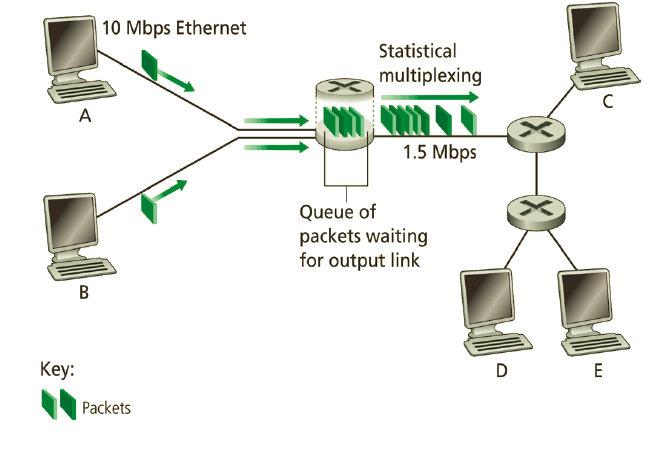
\includegraphics[width=0.8\textwidth]{PSBuffering.png}
\caption{\label{PSBuffering.png}Buffering in a PS Network}
\end{figure}


\subsection{Protocols}
\begin{definition}{\textbf{Protocol}\\}
A protocol is a set of rules that specify interactions between the communicating entities. We can say it is a language talked by \textsc{peer entities} of different devices.
\end{definition}
\begin{definition}{\textbf{Layer}\\}
A layer is a entity that offer services to its upper entity using the services offered by its lower layer entities.
\end{definition}
\begin{definition}{\textbf{Interface}\\}
An interface can be seen as a language talked by \textsc{neighbor} entities of the same device.
\end{definition}
\begin{definition}{\textbf{Embedding}\\}
Embedding is a concept which we refer to when considering the \textsc{Protocol Data Unit (PDU)} of upper layer as the \textsc{Service Data Unit (SDU)} of lower layer.
\end{definition}

\subsubsection{OSI model}
\begin{equation}\text{Host Layers = }
\begin{cases}
\text{\textbf{7. Application}} \Rightarrow \text{\textsc{data}} \\ \rotatebox[origin=c]{180}{$\Lsh$} \text{ Network Process to Application}\\
\text{\textbf{6. Presentation}} \Rightarrow \text{\textsc{data}}\\ \rotatebox[origin=c]{180}{$\Lsh$}
\text{ Data Representation and Encryption}\\
\text{\textbf{5. Session}} \Rightarrow \text{\textsc{data}}\\ \rotatebox[origin=c]{180}{$\Lsh$}
\text{ Inter-host Communications}\\
\text{\textbf{4. Transport}}\Rightarrow \text{\textsc{segments}}\\\rotatebox[origin=c]{180}{$\Lsh$} \text{ End-To-End Connections and Reliability}\\
\end{cases}\\
\end{equation}
\begin{equation}\text{Media Layers = }
\begin{cases}
\text{\textbf{3. Network}} \Rightarrow \text{\textsc{packets}}\\ \rotatebox[origin=c]{180}{$\Lsh$}
\text{Path Determination and IP} \rightarrow \text{Logical Addressing}\\
\text{\textbf{2. Data Link}} \Rightarrow \text{\textsc{frames}}\\ \rotatebox[origin=c]{180}{$\Lsh$}
\text{ MAC and LLC} \rightarrow \text{Physical addressing}\\
\text{\textbf{1. Physical}}\Rightarrow \text{\textsc{bits}}\\\rotatebox[origin=c]{180}{$\Lsh$} \text{ Media, Signal and Binary Transmission}
\end{cases}
\end{equation}

\begin{figure}
\centering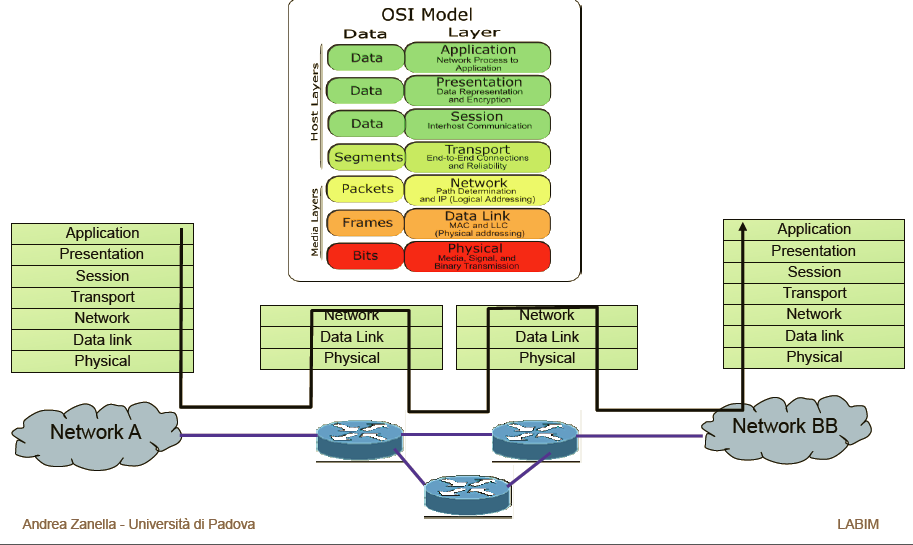
\includegraphics[width=0.8\textwidth]{OSImodel.png}
\caption{\label{OSImodel.png}Protocols accross network elements}
\end{figure}

\begin{figure}
\centering 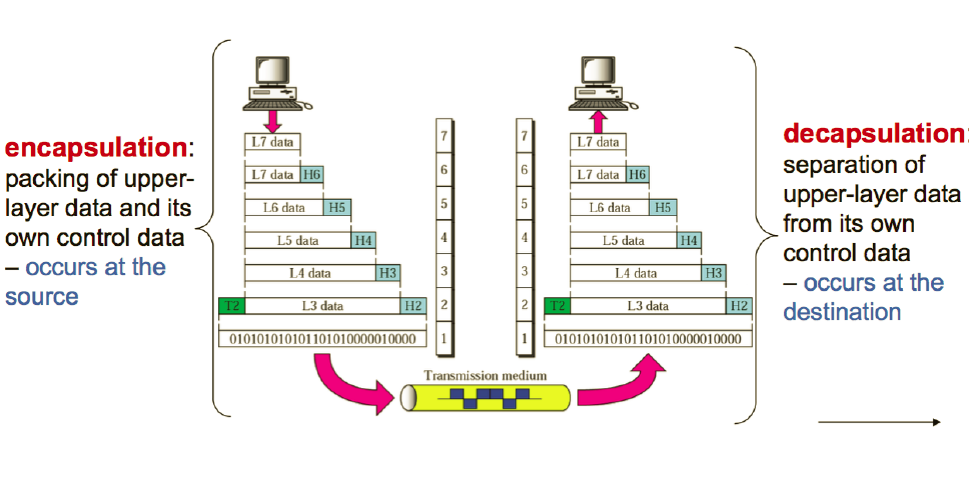
\includegraphics[width=0.9\textwidth]{ENCAPandDECAP.png}
\caption{\label{ENCAPandDECAP.png} Encapsulation and Decapsulation}
\end{figure}

\paragraph{OSI vs TCP/IP}
In the \textit{Internet Protocol Suite}, as we already have said, we have the two most important internet protocols (TCP and IP) and we can model every telecommunication system as the following TCP/IP protocol stack:
\begin{equation}\text{TCP/IP protocol stack = }
\begin{cases}
\text{\textbf{4. Application}} \\\rotatebox[origin=c]{180}{$\Lsh$} \text{ftp, telnet, smpt, http, x-windows}\\
\text{\textbf{3. Transport}} \\\rotatebox[origin=c]{180}{$\Lsh$} \text{TCP-UDP}\\
\text{\textbf{2. Internet}} \\\rotatebox[origin=c]{180}{$\Lsh$} \text{IP}\\
\text{\textbf{1. Subnet}} \\\rotatebox[origin=c]{180}{$\Lsh$} \text{Ethernet, Token-ring}
\end{cases}
\end{equation}

\paragraph{Request for Comments (RFC)}
A Request for Comments (RFC) is a type of publication from the \textit{Internet Engineering Task Force (IETF)} and the \textit{Internet Society (ISOC)}, the principal technical development and standards-setting bodies for the Internet. 

An RFC is authored by engineers and computer scientists in the form of a \textbf{memorandum describing methods}, \textbf{behaviors, research, or innovations applicable to the working of the Internet and Internet-connected systems}. It is submitted either for peer review or simply to convey new concepts, information, or (occasionally) engineering humor.[1] The IETF adopts some of the proposals published as RFCs as Internet Standards.

\subparagraph{Scheme}
This kind of items has to follow the follow scheme:

\begin{equation}\text{Internet Draft = }
\begin{cases}
\text{\textbf{1. Proposed Standard}}\\\rotatebox[origin=c]{180}{$\Lsh$} \text{\textit{1.1 Draft Standard}}\\
\rotatebox[origin=c]{180}{$\Lsh$}
\text{\textit{1.2 Internet Standard}} \\ \rotatebox[origin=c]{180}{$\Lsh$} \text{\textsc{Historic}}\\
\text{\textbf{2. Best Current Practice}} \\ \rotatebox[origin=c]{180}{$\Lsh$} \text{\textsc{Historic}}\\
\text{\textbf{3. Experimental}}\\ \rotatebox[origin=c]{180}{$\Lsh$} \text{\textsc{Historic}}\\
\text{\textbf{4. Informational}}\\ \rotatebox[origin=c]{180}{$\Lsh$} \text{\textsc{Historic}}         
\end{cases}
\end{equation}

\subparagraph{Requirements levels}
\begin{enumerate}
\item Required\\ $\rotatebox[origin=c]{180}{$\Lsh$}$ Must be implemented by all Internet systems (e.s IP and ICMP)
\item Recommended\\$\rotatebox[origin=c]{180}{$\Lsh$}$ Recommended but not required (e.s TCP)
\item Elective\\$\rotatebox[origin=c]{180}{$\Lsh$}$ Not required nor recommended, but feel free to use if you like
\item Limited use\\$\rotatebox[origin=c]{180}{$\Lsh$}$ Use in specific situations only (e.s experimental RFCs)
\item Not recommended\\$\rotatebox[origin=c]{180}{$\Lsh$}$ Not to be used 
\end{enumerate}

\subsection{Application architecture}
There are three types of application architecture:
\begin{enumerate}
	\item \textbf{Client-server}
	\begin{itemize}
	\item Server
		\begin{equation}
		\begin{cases}
		\text{ Always-on host}\\
        \text{ Permanent IP address}\\
		\text{ Server farms for scaling}
		\end{cases}
		\end{equation}
	\item Clients
		\begin{equation}
		\begin{cases}
		\text{ Communicate with server}\\
		\text{ May be intermittently connected}\\
		\text{ May have dynamic IP addresses}\\
		\text{\textbf{ Do not communicate directly with each other}}
		\end{cases}
		\end{equation}
	\end{itemize}
	\item \textbf{Peer-to-Peer (P2P)}\\ \begin{equation}
	\begin{cases}
	\text{ No always-on server}\\
    \text{ Arbitrary end systems directly communicate}\\
    \text{ Peers are intermittently connected}\\
    \text{ Peers change IP addresses}\\
    \text{ High scalable}\\
    \text{ Difficult to manage}
	\end{cases}
	\end{equation}
    
\item \textbf{Hybrid of client-server and P2P}\\
\end{enumerate}














\chapter{Addressing Fundamentals}
An address uniquely identify the source and final destination and specify the route through the networks.
\section{Internet naming and addressing}
\subsection{Requirements}
\begin{itemize}
\item Uniqueness/unambiguity
\begin{equation}
\begin{cases}
\text{1. Every address} \stackrel{shall\, be}{\Rightarrow} \text{ associated to a } \textbf{single} \text{ entity in the network}\\
\text{2. The \textbf{same} entity} \stackrel{may\, be}{\Rightarrow} \text{ multiple addresses}
\end{cases}
\end{equation}
\item Multilevel structure
\begin{equation}
\begin{cases}
\text{1. Allow for hierarchical routing}\\
\text{2. Address shall be \textbf{unique within it scope}}
\end{cases}
\end{equation}
\item Internet $\Rightarrow$ Each address must be unique \textbf{within the scope of the layer}
\end{itemize}

\subsection{Address Level}
\begin{itemize}
\item PHY/MAC address
	\begin{enumerate}
	\item They \textbf{uniquely identify} the 				\textit{Network Interface Card (NIC)} in a local 		network.\\
	\item The strict condition is that \textbf{it must be 		unique at local level}, but in practice we can find 		it is also at global level.
    \item MAC address is \emph{Hardware} written to have a faster process
	\item \emph{Example: } Bluetooth [20-c9-d0-d5-aa-be], 		WiFi [20:c9:d0:d5:aa:bd], Ethernet [a0:4f:d4:4:91:cf]
\end{enumerate}
\item Data Link Layer address (DLL) $\Rightarrow$ Logical Link Control (LLC) address
	\begin{enumerate}
	\item They uniquely identify a logical \textit{point-to-point} connection between two directly connected hosts.
    \item \textbf{Must be unique for reach point-to-point connection}
    \item Can be repeated in different connections
    \item Usually quite short $\rightarrow$ one/two bytes
	\end{enumerate}
\item Network Layer address $\Rightarrow$IP address
	\begin{enumerate}
	\item Uniquely identify a host in the entire Internet
    \item \textbf{Must be unique at global level}
    \item \emph{Example: } only valid network address today $\rightarrow$ IP address: 192.168.13
	\end{enumerate}
\item Transport Layer Address $\Rightarrow$ Port Numbers
	\begin{enumerate}
	\item \textbf{Unique within a host for a given transport protocol}
    \item Ca be re-used in different hosts or in the sam host for different transport protocols $\Rightarrow$ TCP and UDP can re-use the same port numbers
    \item Usually \textit{Transport Layer Address = 2 bytes}
    \item \emph{Examples: } Port Number 21, 22, 23, 25, 53, 80 corresponding to \textit{File Transfer Protocol (FTP), Secure Shell (SSH), Telnet remote login service, Simple Mail Transfer Protocol (SMTP), Domain Name System (DNS) Service, Hypertext Transfer Protocol}
	\end{enumerate}
\item Application Address
	\begin{enumerate}
	\item Human readable mnemonic addresses
    \item \textbf{Unique at global level}
    \item \emph{Examples: } URL or email like www.unipd.it and zanella@dei.unipd.it
	\end{enumerate}
\end{itemize}

\subsection{Address Translation Mechanisms}
One host interface has 3 different addresses: a \emph{Host Name}, readable like "zanella.dei.unipd.it", converted to the \emph{Internet address (IP)} by the \emph{Domain Name System (DNS)} and the conversion of the \textit{IP address} into the \textit{MAC address} due to the \textit{Address Resolution Protocol} (ARP).

\subsection{Addressing in Internet}
\begin{itemize}
\item \begin{equation}{\text{ IP Address = }}
\begin{cases}
\text{ 32 bits}\Rightarrow\text{ Grouped in octects}\\
\text{ Every octects}\Rightarrow\text{ Decimal number} \in \{0,255\}\\
\text{ Every decimal number is separated by dots}
\end{cases}
\end{equation} 
\item IP address = [ IP Network Address $\mid$ IP Host Address ]

$\curarr$ \textbf{IP Network Address} \textbf{$\Rightarrow$} \textbf{Uniquely identify a \emph{Network} in the \emph{Internet}}

$\curarr$ \textbf{ IP Host Address $\Rightarrow$ Uniquely identify a \emph{Host} in a \emph{Network}}
\item \begin{definition}{\textbf{Socket}\\}
A Socket is the combination of the IP address ($\Rightarrow$ Network Layer) and the Port Number ($\Rightarrow$ Transport Layer).

$\curarr$ It represent the \textbf{endpoint of each connection in the internet}: <IP,port>

\end{definition}
\item \begin{equation}
\begin{cases}
\text{ Street} \Longleftrightarrow \text{ IP Network Address}\\
\text{ Building} \Longleftrightarrow \text{ IP Host Address}\\
\text{ Apartment} \Longleftrightarrow \text{ Port Number}\\
\text{ Person} \Longleftrightarrow \text{ One application per port number}
\end{cases}
\end{equation}
\end{itemize}


\section{Transport Service}
There are two types of \emph{Transport Service Protocols}: TCP (Transmission Control Protocol) and UDP (User Data Protocol)

\begin{itemize}
\item TCP: 
\begin{enumerate}
\item \textbf{Connection-oriented transport service} $\Rightarrow$ Host-to-Host connectivity at the Transport Layer of the Internet Mode
\item \textbf{A logical e2e connection is established between the sender and the receiver} processes and is \emph{full duplex}
\item Each endpoint is identified by \emph{<IP,port>}
\item The TCP connection is identified by the sockets of its endpoints
\item 
\begin{definition}{\textbf{TCP socket}\\}
A TCP socket is a pair of sockets as <$IP_A$,$port_A$><$IP_B$,$port_B$>
\end{definition}
\item The Transmission Control Protocol provides a communication service at an intermediate level between an application program and the Internet Protocol.
\item An application does not need to know the particular mechanisms for sending data via a link to another host, such as the required packet fragmentation on the transmission medium
\item \textbf{At the transport layer} of the protocol stack $\Rightarrow$ TCP:
\begin{enumerate}
\item Handles all handshaking + transmission details
\item Presents an abstraction of the network connection to the application
\end{enumerate}
\item \textbf{At the lower levels} of the protocol stack, $\Rightarrow$ due to \textit{network congestion, traffic load balancing, or other unpredictable network behaviour}, IP packets may be lost, duplicated, or delivered out of order $\Rightarrow$ TCP:
\begin{enumerate}
\item Detects these problems
\item Requests re-transmission of lost data
\item Rearranges out-of-order data 
\item Helps minimize Network congestion to reduce the occurrence of the other problems
\item If the data still remains undelivered the source is notified of this failure 
\item Once the TCP receiver has reassembled the sequence of octets originally transmitted $\Rightarrow$ It passes them to the receiving application
\item AT the end TCP abstracts the application's communication from the underlying networking details
\end{enumerate}
\end{enumerate}
\item UDP:
\begin{enumerate}
\item Connectionless transport service
\item There's \textbf{no logical e2e connection}
\item Sender sends the packet to a receiver and that's it
\item it suffices to specify the receiver socket $<IP,port>$
\item
\begin{definition}{\textbf{UDP Socket}\\}
A UDP Socket is just purely <$IP_B$,$port_B$>
\end{definition}
\end{enumerate}
\end{itemize}

\section{Key points}
\begin{equation}{\text{One Host}\rightarrow}
\begin{cases}
\text{ At least 1 IP address} \Rightarrow \text{\emph{A Host can have multiple IP addresses}}\\
\text{ Multiple Processes} \Rightarrow \text{Each process is identified by one port number}
\end{cases}
\end{equation}
\begin{equation}{\text{IP address}\rightarrow}
\begin{cases}
\text{\emph{IP address must be unique in the Network Domain}}\\
\curarr \text{ 		Public Internet} \rightarrow \text{Globally unique IP address}\\
\curarr \text{ 		Private Network} \rightarrow \text{Unique in the private network \textbf{only}}
\end{cases}
\end{equation}

\begin{itemize}
\item The connection is identified by one or more pairs \textit{<IP address,port number>} called \textbf{socket} which are \emph{unique in the network domain}.
\item IP addresses uniquely identify network endpoints int the Internet, except in case of anycast routing
	\begin{itemize}
	\item A public IP address can be associated to  single network endpoint except in case of anycast routing\\$\curarr$
Private IP addresses can be freely re-used in private networks, but cannot be used to route packet through the public Internet    
    \item A single network endpoint can be associated to multiple IP addresses
    \item Host connected to multiple networks \textbf{must} have multiple IP addresses
	\end{itemize}
\item Port numbers uniquely identify an application ina host
\begin{itemize}
\item Well-known port number are assigned to common applications
\item other port numbers can be used to private applications
\end{itemize}
\item A socket \textit{<IP address,Port number>} uniquely identify an endpoint of a logical connection in Internet 
\end{itemize}



\chapter{Data Link Layer}
\section{DLL}
Data Link Layer is the link-layer counterpart of Transmission Control Protocols (TCP) and provides several services as we discuss in the following subsection.
\subsection{Services}
The services performed by DLL are:
\begin{enumerate}
\item \textit{Link-Layer connection} set up/teardown
\item \textit{Logical link} set up $\rightarrow$ \textit{Exchange control messages} for negotiation of logical link characteristics
\item \emph{Synchronization} $\rightarrow$ \textbf{Division of the bit stream provided by PHY layer in characters and frames}
\item \emph{Segmentation and Reassembly} of upper layer Information Units $\Rightarrow$ Suitable MAC frame units
\item \textit{Flow Control} $\rightarrow$ Not necessarily provided
\item \textit{Error Control }$\rightarrow$ Not necessarily provided
\item \textit{Medium Access Control} $\rightarrow$ Not necessarily provided
\end{enumerate}

\emph{Example 1:} DLL has to recognize there is another Bluetooth device in the network. To do so it has to find  the \emph{signature} corresponding to that particular device that is needed in order to communicate.

In Bluetooth every node change the transmission frequency at every packet according to a certain pattern and \textbf{this pattern depends on the device}.

In order to set up a communication between two devices is has to be performed a procedure that allow them both to share the same pattern. All of these operations are performed by the Data Link Layer. 

\emph{Example 2:} Ethernet technology 

Medium Access Control is needed when there are multiple nodes that use the same link (Wi-Fi)

\subsection{Addressing}

The different layer define different addressing spaces and that are defined basing on the specific purpose of that layer.

Ethernet and Bluetooth could have the same mac address, is it a problem? In the IP layer there can't be two host with the same address but the addresses need to be unique within the scope of the layer. Bl and Et speaks different languages so they don't collide wit each other.

Each network interface cards in the world have different mac addresses

\section{ARP}
\subsection{IP encapsulation}

Pag. 6) The source and the destination belong at the same net so there's no need of routing $\Rightarrow$ In this case the hosts have the same prefixes. 

ARP table where for every possible IP address in the same local net maintain the same local address of the host

Pag. 8) The source and the destination IP address belong to the source and the ultimate node itself, but the MAC destination address is the MAC address of the router in the first communication

TE MAC ADDRESS HAS A POINT-TO-POINT SCOPE

The IP datagram becomes the payload at the physical layer

\subsection{Address Resolution Protocol}
\paragraph{Example of \emph{directed connection}}
ex) src B doesn't know the mac address of A
arp request is a request that carries inside of his pck some information of the mac address of the sender and the receiver.
The ARP request the IP and the MAC address of the source

the reply is not broadcasted because node A knows how to reach node B once the ARp request from B arrived to A

\subsection{ARP packet format}
The arp request and reply hve the same size, in the arp req the mac addr field is set zero because the sender doesn't know the mac addr of the receiver, but why they should be of the same size? Possibility

Is to simplicity because to design a protocol is easier to manage things that are constant in time $\Rightarrow$ efficiency of the processing, processing is the main problem 

ARP PDU:[SRC MA|SRC IP|DST MAC|DST IP] $\stackrel{\text{Embedding}}{\Rightarrow}$ Phy payload at which we add the PHY Header

PHY Header: [SRC MAC|BROADCAST(111...11)]

\subsection{Proxy ARP}
proxy is a piece of software that pretends to be something it is not, interien in the flow pretending to be a souurce. 
In the exmple he tries to replay to the added subnets 
The router splits the broadcasting domain 

If NO PROXY ARP, the host has to know that the adde subnet belongs to a different network 

the use of the proxy let the host to send an arp request ad plays the role of an etire subnet. The higher interface pretends to be the subnet that contain the host and that is trying to send the arp request, the lower interfaace plays the role of the subnet destination of the request. 

the proxy = I'M THE GUY YOU'RE LOOKING FOR

\paragraph{Another se of the proxy arp}
The trick is to put the ip address of all the nodes to zero pretending their to be part of the same local area network (LAN)

\subsection{Reverse ARP}
Is sent broadcasted but is repy by just one host

\subsection{Fun Facts}
\begin{itemize}
\item In multi-hop connection IP addresses do not change in general, exception is made for we use other protocols, while MAC addresses change. THis is for the fact that IP address has local meaning.
\item ARP/RARP requests are sent to the broadcast MAC Address (sent in a \textit{broadcast way}) and the ARP/RARP replies as \emph{unicast}
\item ARP request do not cross routers, the router pretend to be the sender of the request or the destination of it. The request stops at its interface and he plays the role of collecting the dots
\end{itemize}

\chapter{Error Control}
We say that the DLL can provides different services to different layers.
At upper layer DLL offered services can be reliable (retransmit pck received with error until it is correctly received or until a certain number of attempts have been made) or reliable. 

Unreliability stands for some clue concepts:
\begin{equation}{\text{Unreliable service of DLL}\rightarrow}
\begin{cases}
\text{\textit{ Error transparent} service} \rightarrow \text{ very rare}\\
\text{ \textit{Silent Packet Dropping} mode} 
\end{cases}
\end{equation}

This means that at the upper layer we know either a pck is received or it is entirely not. 

To provide \textit{error control} and \textit{reliability} at DLL we need: 
\begin{enumerate}
\item \textit{Error control} $\Rightarrow$ We need a field in the header of the PDU that makes it possible to check for bit errors, a way to recognize if the received pck contains error or not

At DLL we do not correct errors whereas of the PHY layer we use a redundancy to correct the misleading information. This is due to the fact that, if we receive a un-correct pck to the DLL it means it contains several errors because the control errors code 
\end{enumerate}

\paragraph{Cycle Redundancy Check (CRC)}
DLL: [SRC MAC|DST MAC|Type|...|Payload|Control Field = CRC]

The CRC code is generated by the hardware while the pck are being transmitted


\section{Review of Coding}

Let we consider a domain set of Information words $\bar{a} = [a_0,a_1,...,a_{k-1}]$ with cardinality $2^k$. The codeword co-domain will be a $2^n$, with $n > k$, made by $\bar{c} = [c_0,c_1, ..., c_{n-1}]$.
If we assume there are errors in the transmission if we received a codeword which has no information word corresponding to it.

\begin{definition}{\textbf{Codebook}\\}
The codebook is the collection of codewords of n bits associated to valid information words. WIth ths definition the cardinality/size of the codeboo is $2^k$
\end{definition}
\section{Yuri's notes of this lecture }

\section{SLL}
Overview of past concepts:
\begin{itemize}
\item Generator polynomial : $g(x) = g_0 + g_1 ì ... + g_{r-1}x^{r-1} + x^r$
\item Code: $C = {g(x)a(x) : deg(a) \leq n - r - 1}$
\item $x^n-1 = g_1(x)\cdot g_2(x)\cdot ... g_k(x)$ where $g_i(x)$ are monic and irreducible then any $g_{i_1}(x)\cdot g_{i_2}(x)\cdot ... g_{i_m}(x)$ with $i_1, i_2, ... i_m \in \{1.2.... k\} \Rightarrow$ $g(x)$ is a generator polynomial of a cyclic redundancy Code of length $n$ 
\item $I \subseteq F[x]$ such that I is closed under moltiplication with polynomial $s \in F[x] \Rightarrow$ I is \emph{Ideal} such that, with $g \in F[x]$, $I = \{f(x)g(x) : f(x) \in F[x]\}$  
\end{itemize}

\subsection{Exercise}
Hyp: n = 7
\begin{equation}
x^7 - 1 = x^7 + 1\\
\end{equation}
 We identify the first factor, we divide $x^7 - 1$ by this factor 
\begin{equation}
x^7 - 1 = (x - 1)(x^6 + x^5 + x^4 + x^3 + x^2 + x + 1)
\end{equation}
We try to find a divisor for the second term. We try $x^2$ and $x^2 + 1$ or also $x^2 + x + 1$. To find if it is a divisor we have to calculate if the rest of the division between the term and itself is zero  
\begin{equation}
x^6 + x^5 + x^4 + x^3 + x^2 + x + 1 = (x^2 + x + 1)(x^4 + x) + 1
\end{equation}
We see that this division gives a rest that is non-zero. 

We now try with the divisors of degree 3 like $x^3$, $x^3 + 1$ or $x^3 + x + 1$. We find nether they are divisor for the last term so we try with $x^3 + x^2$ and $x^3 - x^2 - 1$ etc.

The final solution is
\begin{equation}
x^7 - 1 = (x - 1)(x^3 - x^2 - 1)(x^3 + x - 1)\cdot 1
\end{equation}

\subsection{Parity Check Code}
Given a $g_1(x) = x + 1$ \emph{Parity Check Code}.

We know that \textbf{every cycle redundancy codeworks of....}

A codewords generated by this polynomial can be $c_1 = \{a(x)g_1(x): a(x) = a_0 + a_1x + ... a_{n-2}x^{n-2}\}$. 
If $a = [a_0 ... a_{n-2}] \rightarrow a(x) = a_0 + a_1x + a_{n-2}x^{n-2}$, that, combined with $g_1(x)$, result in $c(x) = a(x)g_1(x) = a(x) + xa(x) = [a_0, a_1+a_0, a_2+a_1, ... a_{n-2}]$. Overall we'll have $n$ bits but in this expression we'll not recognize a parity check code because this one shown is not systematic.

\begin{definition}{\textbf{Systematic Code}}

A cycle code is \emph{systematic} if 
$\forall a \rightarrow \underline{c} = [\underline{s},\underline{a}]$

Dimensionally $[a] = n - r$ bits, $c$ will have $n$ bits and $[s] = r$ bits
\end{definition}
 
 We can write 
 \begin{equation}
 x^n - 1 = g_0(x)g_1(x)1dots g_k(x)
 \end{equation}
 And we want to choose $g(x)$ such that $deg(g) = r$ with $r$ is the number of redundancy bits to append to the information words. Remembering that $g(x)$ generates the code $C$
\begin{equation}
\forall a \rightarrow \underline{c} = [\underline{s},\underline{a}]\\
c(x) = s(x) + a(x)x^r \in C
\end{equation}

We wish to find $s(x)$, $deg(s) \leq r - 1$ such that $s(x) + a(x)x^r$ is a multiple of g(x).
\begin{equation}
\text{Find} s(x) \rightarrow \exists q(x) s.t s(x)+a(x)x^r = g(x)q(x)
\end{equation}

Let $r(x)$ be the residual of the division of $a(x)x^r$ by g(x) such that $a(x)x^r = g(x)\widetilde{q(x)} + r_o(x)$. 

The important is that $deg(r_o(x)) < deg(g) = r$. SO we can write 
\begin{equation}
a(x)x^r + r_o(x) = g(x)\widetilde{q(x)}
\end{equation}
The solution is to take $s(x) = \text{residual of } \frac{a(x)x^r}{g(x)}$.

So the process can be sum up as follows:
\begin{enumerate}
\item Given $\underline{a} = [a_0, ..., a_{n-r-1}]$
\item Compute $b(x) = a(x)x^r \Rightarrow \underline{b} = [000...0,a_0,a_1,...a_{n-r-1}]$, which is a shifted vectors with part dimensions $[000...0] = r$ zeros and overall $n$ bits
\item Compute the residual of the division of $b(x)$ by $g(x) \rightarrow s(x)$ with $\underline{s} = [s_0,...,s_{r-1}]$
\item $c(x) = b(x) + s(x) \Rightarrow \underline{c} =  [s_0, s_1, ..., s_{r-1},a_0,...a_{n-r-1}]$
\end{enumerate}

\subsection{Reception}
The sender sends the vector $a(x)$, which it coded like $c(x)$. The channel take the transmitted codeword and operates an operation adding $\underline{e} = [e_1,...,e_n]$ where $e_i = 1$ if the $i-$th received bit is $\neq i-$th transmitted bit and $e_i = 0$ otherwise.

The receiver get $R(x) = c(x) + e(x)$, with $R_i = c_i \bigoplus e_i$. It checks whether $R(x) \in C$ and if is multiple of g(x). It compute $R(x)$ dividing it by $g(x)$ and getting $q(x)$ as result with residual $r_o(x)$. 

If $r_o(x) = 0$ then the word $R(x) \in C$ and is accepted, otherwise it is rejected. 
\begin{equation}
If e(x) = 0 \rightarrow R(x) = c(x), \underline{R} = [R_0,R_1,...,R_{n-1} and \underline{c} = [s_0,s_1,...s_{r-1},a_0,a_1,...,a_{n-r-1}]
\end{equation}
In this case ($e(x) = 0$) the word is accepted $\underline{R} = \underline{c}$ and $\widetilde{a} = [R_r,R_{r+1},..R_{n-1}] = \underline{a} = [a_0,a_1,...,a_{n-r-1}]$

If $e(x) \in C - {0}$ then R(x) is divisible by g(x) and gets accepted $\Rightarrow$ undetected error patterns

\section{Single errors}
In \emph{Single errors} $e(x) = x^h$ where h is the position of error bit and $\underline{e} = [00...01000]$ with the item $1$ in the $h$-th position. 

So we have to find g(x) s.t $x^h$ is not divisible by g(x). 
\begin{theorem}
Any g(x) with more than 1 non-zero coefficient generates a code that can detect all single errors. 
\end{theorem}

\paragraph{\underline{\textbf{Proof}}}
$g(x) = x^m + \widetilde{g(x)} + x^r$, with $m < r$. 

$e(x) = x^h$ for any $h \leq n - 1, x^h$ canot be divided by g(x) with zero-residual

If $h < r$ the solution is obvious.

Else $h > r$ by contradiction $\exists q(x)$ s.t $x^h = q(x)g(x)$ and $q(x) = x^{h-r} + \widetilde{q}(x) + x^j$. 

We now have $(x^{h-r} + \widetilde{q}(x) + x^j)(x^r + \widetilde{g}(x) + x^m) = x^h$ and we multiple the two term in the left as follows
\begin{equation}
x^r\cdot x^{h-r} + x^r(\widetilde{q}(x)+x^j) + \widetilde{x}(x^{h-r}+\widetilde{q}(x)+x^j) + x^{m+h-r} + x^m\widetilde{q}(x) + x^{m+j} - x^h = 0
\end{equation}
Where the last term $x^h$ can be deleted. 
The statement we made is false and so $x^h$ can't be divided by $g(x)$

We can see that $x^{m+j}$ is the term with the least degree above all and doesn't simplify. By construction $h - r > j$ and by definition $m$ is the degree of $g(x)$.

In conclusion we can say that $g(x)$ built the way we had is not a possible divisor of $x^h$

\textbf{FINE-METTI IL QUADRATINO}

An error sequence $\underline{e}\neq 0$ is undetected when e(x) is multiple of g(x).
All error patterne swith a single error ($e(x) = x^h$) are aòways detected by a CRC generated by polynomials with more than one term. 


COnsidering g(x)= x + 1 code with n where, n - 1 is the size of information word and n the size of codeword. We also said that $x^n + 1 $ can be written as a linear combination between monic (monomi?) as $x^n + 1 = (x+1)...$.

\paragraph{Systematic Codeword}
To obtain 
\begin{enumerate}
\item $b(x) = a(x)\cdot x^r \stackrel{g(x) = x + 1 	AND r = 1}{\rightarrow} b(x) = a_{n-2}x^{n-2} + a_{n-3}x^{n-3}+...+a_0x$
\item Divide b(x) with g(x) getting $b(x) = q(x)g(x) + s(x) \rightarrow a_{n-2}x^{n-2} + a_{n-3}x^{n-3}+...+a_0x = (x + 1)(a_{n-2}x^{x-2} + (a_{n-2} + a_{n-3})x^{n-3}) + (a_{n-2}+a_{n-3}+a_{n-4}+..a_0)$
\end{enumerate}

A parity check can detect single errors or odd error bits as we can find out with the following theorem
\begin{theorem}
All error patterns with odd number of errors are always detected by polunomial with even number of terms.
\end{theorem}

It's also true that every polynomial with even numbers of terms is a multiple of (x + 1). 
In other words we can use an example to remark that every pattern with 2 errors can be detectd by a polynomial with 3 terms. 

It's sufficient and necessary to have a polynomial with an even number of terms to detected a pattern with odd number of erros. The theorem says that every genertor polynomial is multiple of (x + 1) so every $g(x)$ with an even number of terms can be written as $g(x) = (x+1)+...$.

Let the error be $e(x) = x^h$ and $\varepsilon$ the probability of having an error in the considered patter.
The probability of having 3 errors will be ()
\begin{itemize}
\item $e(x) = x^h \rightarrow \sim \varepsilon\cdot(1-\varepsilon)^{n-1}$
\item $e(x) = x^h(11 + x^j + x^e) \rightarrow \sim \varepsilon^3\cdot(1-\varepsilon)^{n-3}$ (binomiale n su 3)
\item $e(x) = x^h(1  x?j + x^e + x^m + x^v)  \rightarrow \sim \varepsilon^5\cdot(1-\varepsilon)^{n-5}$ (binomiale n su 5)
\end{itemize}  

We want to find all error patterns with only 2 erros. 
$e(x) = x^h + x^{h+m} = x^h(1+x^m) \Rightarrow$
Any g(x) with more than one non-zero coefficiet can recognize all single errors so that $x^h$ is not a multiple of g(x).

The condition we need to respect to detect all errors patterns with 2 errors in  codeword of $n$ bits is that g(x) must \textbf{not} be a factor of (1 + x^{m}), with $m \leq n - 1$.

If we consider the generator polynomial $g_2(x) = (1 + x)$ it can detect all \emph{odd} errors but not the \emph{even} ones. Also we can say that $g(x) = x^15 + x^14 + 1$ can detect all \emph{2} errors in codewords of size up to $n = 32767$ and also all single errors (because $g(x)$ has more than one term) and all pairs of errors. 

\subsection{Error Burst}
An \emph{error burst} of size $m$ is a sequence of $m$ bits detected randomyl, some of them could be wrong and some not. 
In this case we have $e(x) = x^h(1 + e_{h+1}x + e_{h+2}x^2 + ... + e_{h+m}x^{m-3} + x^{m-1})$ and say that h is the position of the first error, the last bit is also wrong and the other are unknown.

We can say so that $e(x)$ can be recognized by a $g(x)$ such that $g(x) = 1 + g_1x + ... + g_{r-1}x^{r-1} x^r$ with $r > m-1$.

In general a generator polynomial of degree $r$ and with form $g(x) = 1 + ... + x^r$ can detect all error bursts of length $m \doteq r$.

\section{Review of ARQ}
ARQ can be
\begin{itemize}
\item S&W $\Rightarrow$ Tx WIndow = 1 pck, Rx WIndow = 1 pck
\item Go-Back-N $\Rightarrow$ Tx windows = N pcks, Rx windows = N pcks
\item Selective Repeat $\Rightarrow$ Tx windows = N pcks, Rx windows = M pcks
\subsection{Stop & Wait}
\subsection{Go-Back-N}
\subsection{Selective Repeat}
\textbf{INSERIRE DISEGNO}
Assume packet 5 is lost. There'll be a gap in the receiver input so that the pck after the one has been lsot will be stored at the MAC layer of the receiver.

The receiver will send multiple ack(5). During \emph{Retransmission Time}the ack of the pck lost will be continuously sent, after the \emph{Retransmission Timeout}(RTO) the pck has been lsot has to be retransmitted (pck 5 in i.e).

Every single pck can have its own timer that runs in parallel with the others. 

Options of implementation:
\begin{enumerate}
\item Keep one RTO per Tx window $\Rightarrow$ It refers the timeout at which the first pck has to be retransmitted. 
Every time we have the ack of a new pck, the RTO starts again. 
If you have ack of a pck that has already been sent, the RTO keeps running.
\item Keep one RTO per pkc AND the receivers sends acks that will be \emph{selective} $\Rightarrow$ the ack will says: "I received everythin up to 6 but I have a gap between 4 to 6". In this case the implementations is more efficient in some situations but surely is more informative.   
\end{enumerate}

\paragraph{Example}
Hyp:
\begin{itemize}
\item Tx windows = 4 pcks
\item Pipe capacity = 4 pcks
\end{itemize}

Suppose to have 4 pcks to be sent and we have Tx window = Pipe capacity. If everything goes right we have a continous flow of received pcks and after the deliver of pck 4 we'll have the ack of receveide pck 1(ack(2)). If I now have pck 5 to be sent,the winodw will be full and i will get back the ack(3) (received pck 2). 

So if I correctly received pck 1 I will received ack(2). Suppose now that pck 2 contains errors and it is not correctly received and the ack pck is not sent back. Pck 3 is correctly received but out of order as for pck 4 and 5 (the're sotred at mac layer and not put at the upper level). 

Duting the RTO the tx window is full so we have to wait for retransmitting pck 2. 
$\spadesuit$

Let us consider an example where the tx windws $\gg$ pipe capacity. This let \emph{idle times} that are due to suboptimal setting of: 
\begin{itemize}
\item RTO is longer than RTT $\Rightarrow$ some performance might be lost because of delayed reaction
\item Tx window size is too small $\Rightarrow$ if we increase it we can transmitt during the phase we're getting back multiple ack of one pck lost. 
\item queuing delay
\item Memory occupied by the pcks in the receiver and the transmitter
\end{itemize}
Remember that the Pipe capacity is somthing that you can not change and depends to the technology you're using.

\section{Performance Analysis of ARQ}
Assumptions we have to consider are:
\begin{enumerate}
\item Long-term average throughput: S
\item Packet delivery delay: D
\item RTO = RTT
\item Bit rate of bottleneck is constant = R
\item Pcks have fixed size: L
\item Acks have fixed size: H 
\item Pcks loss occurs with equal probability: $P_L$
\item Pck is correctly received with probability $P_C = 1 - P_L$
\item Pck errors are iid
\item Connections are not shared between flows
\item Acks are \emph{always successfull} so they're always correctly received  
\end{enumerate} 
Acks are sent at lower level with high probability to achieve robustness. 
In classica communication data pcks are huge (1000 bytes) and the acks are few bytes. If the acks is not correctly recevide the receiveer has to resent thousands of bytes and this is a waste of time and performance. So the last one assumption is crucial.   
 
\subsection{ARQ S&W}
A \emph{renewal reward processes} is characterized by a sequence of \emph{interarrival times}$\{A_i\}$ that are iid. 

Every statistical dependencce of the past is deleted after an interval $A_i$ has occured.

Let us define \emph{rewars}$\rho_i$ assigned to interval $A_i$.

The long-term average reward rate tends to $\frac{E[rho_i]}{E[A_i]}$. 

In our protocols the rewards are the numbers of pck deliver to the destination and the $A_i$ is the time that occured to do so. 


\textbf{INSERISCI DISEGNO}
We said that RTO = RTT so every intervals are the same and between the 2 pcks does not happen anything so RTT ar renewal time. 
So we can say that
\begin{equation}
\begin{cases}
RTO = RTT\\
A_i = RTT \forall i\\
rho_i = \text{ number of bits correctly received in }A_i
\end{cases}
\end{equation}

$rho_i$ is a r.v and can assume 2 values:
\begin{equation}
\begin{cases}{rho_i}
L \text{ If pck is correcly received}\\
0 \text{ if pck is lost}
\end{cases}
\end{equation}


\begin{equation}
\begin{cases}
S_{SW} = \frac{E[rho_i]}{E[A_i]} = \frac{L\cdotP_c + 0\cdotP_L}{RTT} = \frac{L\cdot P_C}{RTT}\\
C_{SW} = R\cdot RTT\, [bits] = \frac{R\cdotRTT}{L}\, [pcks]\\
\frac{L}{RTT} = \frac{R}{C} 
\end{cases}
\end{equation}
$\Rightarrow$ The throughput will be
\begin{equation}
S_{SW} = \frac{R\cdot P_C}{C}
\end{equation}
If C is small (close to 1) the S&W paradigm is fine. 
For the end to end delay D the computation is again simple and wwe look at what happens between the source and the destination. In order to deliver pcks successfully the times we need is $\tau_p ì \frac{L}{R}$. Suppose a pck is lost and the delay $d_{SW}$, which is a r.v, is equal to
\begin{equation}
d_{SW}= r \cdot RTO + \frac{L}{R}\cdot \tau_p = \text{ time of retransmission + time of the successful transmissions}
\end{equation}  
With $r$ the number of retransmissions and $d_{SW}$ is a geometric random variable.

In this case we have:
\begin{equation}
D_{SW} = E[d_{SW}] = \frac{L}{R} + tau_p + RTO\cdot\frac{1-P_C}{P_c} \stackrel{RTO = RTT}{\rightarrow} D_{SW} = \frac{L}{R} + \tau_p + RTT\cdot \frac{1-P_C}{P_C}
\end{equation}

RTO = RTT is no longer true in a end to end communications becuase in this case the RTT will be a random variable. 
\subsection{ARQ GBN}
GBN protocol with the tx windows = N pcks. 
If pck are correctly received every $T = L\R$ we received nother one. assume now that some pcks are lost. I this case the following correctly received pcks will be stored at the MAC layerof the receiver. 
If you have a pck lost the renewal process time will not start just after and so \emph{if TX windoes(n) = pipe capacity and RTO = RTT} 
\begin{equation}
\begin{cases}{A_i = }
\frac{L}{R},\,  \text{if the pck is successfull}\\
N\frac{L}{R} = RTO = RTT \, \text{if pck is lsot} 
\end{equation}
\begin{equation}
\begin{cases}{rho_i = }
L,\, \text{if the pck is successfull}\\
0, \, \text{if pck is lsot} 
\end{equation}
The throughput will be:
\begin{equation}
S_{GBN} = \frac{E[rho_i]}{A_i} = \frac{L\cdot P_C}{L\R\cdot P_c + NL\R(1-P_C)} = \frac{L\cdot P_C}{L\R\cdotP_C + RTT(1-P_C)} = \frac{R\cdot P_C}{P_C + R\L\cdot RTT(1-P_C)} \stackrel{R\L\cdot RTT(1-P_C) = C}{\rightarrow} S_{GBN} = \frac{R\cdot P_C}{P_C + C(1-P_C)} 
\end{equation}
The GBN is good when the $P_C$ is good 

\subsection{SR}
In this case the TX window will be large, the process reniew itself at every step so $A_i = \frac{L}{R}$ and \begin{equation}
\begin{cases}{rho_i = }
L, \, \text{if the pck is correct}
0, \, \text{otherwise}
\end{equation}

The throughput will be
\begin{equation}
S_{SR} = \frac{E[rho_i]}{E[A_i]} = \frac{L\cdot P_C}{L\R} = R\cdot P_C
\end{equation}

\chapter{MAC}
\begin{itemize}
\item Deterministic protocols: All the mac protocols where the access to the medium is predetermined. 
\item Random MAC protocols: In order to transmitt you have to conquer the medium (random strategy). One node does not know how many nodes exist that thave to transmit so they try to transmit 
\item Demand based protocols: something in between. We can't predict which unit will uses the medium, but this strategy allow sthe unit to ask for the medium. SLightly more complex because they requeired combination among all
\end{itemize}

The mac layer is in charge to the delivery of the PDU provided by the upper layer and needs to manage the access to the medium. 

Improtant to notice that DLL is divided in LLL(Logical Link Control) and MAC 

\paragraph{Static Allocation}
Has been skipped
\section{Deterministic protocols}
\subsection{FDMA}
The channel provides a bandwidth and a maximum capacity such tat: $R \backsim B\log_2 (1+\Gamma)$

Split the bandwidth of the channel in subband = subchannel that are fiven to one specific user.  In this case the bit rate is divided among all bt the users can transmitt during all the time, just through some fraction of the bandwidth

To avoid collision you let some space between the subband in which the system will be idle (gap bands). So that each subchannel will have a band < B/3. 

\begin{equation}
\begin{cases}
B_i < \frac{B}{N}\\
R_i \approx \frac{R}{N}
\end{cases}
\end{equation}

\subsection{TDMA}
All the bandwidth to one user but just for a fraction of time. 
SO every user can transmitt with the full bit rate but can do that only for a specific amount of time (slot). 
 
 
\emph{Frame} is a set of N slot after which every user is scheduled again

In case of averagebit rate, which solution is the best one? 
Let's consider the ideal case where you can split the time (TDMA) and the frequency (FDMA) perfectly. 
In terms of longterm the bit rate the throughput is the same $R/N$. 

With FDMA we have the advantage that we don have to wait to transmitt. To do so you have to modulate the signal with different carrier. 

In terms of average system time the time taken from the first pack to start being transmitted to the nd of transmission is slower for TDMA. When you access the channel your pck is transmitt with a higher speed (R) than in FDMA (R/N).

If my pck is L bits long, for TDMA $T_{slot} = \frac{L}{R}$, $delay = \frac{N}{2} T_{slot} + T_{slot} = (N/2 + 1)T_{slot}$

In FDMA the delay will be $= L/R_i = L/R\times N$

\subsection{CDMA}
The suer will share both time and frequency dimension but will use signature for their signals. Every user will uses a different pattern of \emph{chips}(sequences made of on/off phases) to modulate their signal. 

Considering our signal, if it is 1, the trasmitted signal will be the opposite of the chip pattern. WHen our signal becoms 0, the transmitted one will have during that time the same form of the corresponding chip. 

WHen you integral the energy of the signal for a bit period where the original signal values 0 the transmitteed signal matches perfectly with the pattern and the integral will get a postiive peak. In positive bit period for the original signal the energy integrated will get a negative peak. 

\paragraph{Esempio}

2 users. User one assigned to the chip pattern : +1 +1 +1 +1 while user2 is assigned to a different chip pattern: +1 -1 +1 -1.

SUppose that user1 want to transmitt the data seq: $1\, 1 = b_0 b_1$.

After CDMA modulation the first signal corresponding to usr1 will be: $1\,1\,1\,1\,1\,1\,1\,=\,b_0\,b_1$

USer1 want to transmit the data seq: 0 1 --> $-1\,+1\,-1\,+1\,+1\,-1\,+1\,-1\,=\,b_0\,b_1$

SO these 2 signals will be modualtedand sent over the channel that will introduces some attenuation $(\alpha, \beta)$ and assuming any error. Te 2 signals in one channel overlap and the receiver will receive:

$\alpha - \beta \alpha + \beta \alpha - \beta \alpha + \beta \alpha + \beta \alpha - \beta \alpha + \beta \alpha - \beta = r0\, r1\, r2\, r3\, r4\, r5\, r6\, r7$

We act a convesion S/P that produce a pattern of 4 chips = r0 r1 r2 r3 and another conversion tht get r4 r5 r6 r7. 

This paradigm can be seen as communication among people that speak diffrent language. Those who know one language can talk and understand but the listen the speaking of a language they dont know and received that as a "rumore di sottofondo" (noise). 

The spreading sequences should bemade in order to have a poor correation with a cyclic shift of themselves. 



Multipath self-interference = This is a phenomenon called "fading".



CDMA can be implemented in 2 ways: 
\begin{itemize}
\item Direct Sequence Spread Spectrum (DSSS): the price tha tyou pay in order totransmitt 1 single bit of information you actually need to send over the cahnne la sequence of chips (let's say k chips). Since this transmission has to take the same time of the bit and this measn that Tchips = Tbit/k and the signla bandwidth is k time larger than hat required by the original message (information signal) --> it's require a larger bandwisth and it's called spread spectrum because it spreads the bandwidth.    

If the received energy per chip is $\varepsilon$, so thtat the SINR before despreading is $\varepsilon/N_0$, after despreading the enery will be $k\varepsilon/N_0$. In this mode can transmitt using very low power. 

Frequency Hopping Spread Spectrum (FHSS): if the bandwidth of my original signal is B $\backsim 1/Tbit$, you split the KB bandwidth    
\end{itemize}

\section{Random access protocols}

ALOHA has the problem of stability

\subsection{Batch resolution problem}
Pcks arrive in batch (groups) so that the packet arrival process will be a sequence of burst of pcks and then nothing, groups of packs then nothing.

\subsubsection{Splitting-tree BRAs}
The time is slotted with fixed or not sixed.

Some nodes are activated  so they can transmitt, the thers are kept silence

3 situations:
\begin{itemize}
\item no node transmitt : idle slot
\item copia slide
\item copia slide
\end{itemize}

\subsubsection{Recursive resolution procedure}
\paragraph{Diving a batch in subgroups}
This protocol has some drawbacks. 

Avoid the activation of a slot if his neighbor is idle and his parent has collided.

\subsubsection{Splitting Tree Performance Analysis}
batch size: numerb of ndeos in the batch

Average resolution time for a batch size n: T(n) = mean numebr of slot that we need to ersolve the n-problem batch

Throughput: S = n/T(n)

Given n, what we need t determine is the expression of T(n).
Let p be the probability of choosing the left subset (L) after a collision, so 1-p is the probability to chose the right one (R).

A simpel way to find the expression of T(n) is to exploit the recursion:
T(0) = 1; 
T(1) = 1;
Recursion: suppose that you know the expression of T(k) or all k < n and you want to find T(n). 

For n > =2 T(n) = 1 (collided) + E[T(l)] (= n nodes choose L) + E[T(n-l)] ( = n-l nodes choose R)  with l is a random variable (l $\backsim B(n,p)$)
so $T(n) = 1 + \sum\limits_{h = 0}^{n} Pr[l=h](T(h)+T(n-h)) = 1 + \sum\limits_{h=0}^{n} \binom{n}{h} p^h(1-p)^{n-h} (T(h)+T(n-h)) = 1 + \sum\limits_{h=1}^{n-1} \binom{n}{h}p^h(1-p)^{n-h}(T(h)+T(n-h)) + (T(0)+ T(n))(p^n - (1-p)^n) $

So $T(n) = \frac{1 + \sum\limits_{h=o}^{n} \binom{n}{h} p^h(1-p)^{n-h}(T(h)+T(n-h)) + T(0)(p^n+(1-p)^n)}{1-p^n-(1-p)^n}$ 

This is the recursive expression of T(n).



\subsection{CSMA}

the signal takes some time to propagate, the vulnerability interval is tiny.

If the channel is busy:
\begin{itemize}
\item keep in line (wait for the channel): if 2 nodes activate during the channel is busy, the wait but start to transmitt at the end of the previous transmission --> high traffic
\item At the end of the transmission that makes the channel busy the nodes can generate a random backoff. After this backoff the node check the channel, if it's busy the nodes waits for the double time of the random backoff
\end{itemize}

If the node wait time tau and after tau the channel is idle, the node flip a coin and with probability p it transmitt and with probability 1-p it waits a random backoff time
\paragraph{CSMA/CD}
Collision Detection is only in technologies that perform transmission and reception simultaneously (not wireless communication).  


\subsection{CSMA: throughput analysis non-persistent}
All packs have size L and Tx has bit rate R.

Packet arrivals can be modelled as a Poisson Process of rate $\mu [pack/s].$

Goal: We want to find the long term throughput as a function of $\mu$.

$(bit per seconds) S*$

(normalized version) $S = S*\times T \rightarrow$ number always <1 (we can't do bettter than transmitting 1 packet per period). It reaches the vlaue 1 if we perform the perfect MAC

How do we compute the long term throughput? We observe what happens on the channel over time you'll see we have some arrivals according to a Poisson process; if the transmission find the channel idle the transmission will go from t0 to to+T and the signal will occupy the channel for an extra time called $\tau$ = propagation time. So the channel will be busy for an overall time = T + $\tau$. 

The second arrival can be far away from the first one and it can find the channel idle and stars the transmission. It will starts to transmitt with a delay y so that the next process could colldes with it. In this case the busy period will be equal to T + $\tau$ + y.

If we have other arrivals during this last busy period, they'll be stored and they'll start after the previous transmission is over. The sttatistica distribution of the period (busy,idle) is:

Our renewal period: Bi + Ii (Busy period + Idle period)

Reward: 
\begin{equation}{w_i}
\begin{cases}
L \, \text{if tx is successful}\\
0 \, \text{in case of collision}
\end{cases}
\end{equation}

Applying the renewal reward theorem we can say that:
\begin{equation}
S* = \frac{E[w_i]}{E[B_i+I_i]} =\frac{LP_{nc}}{\hat{B}+\hat{I}} 
\end{equation}
WIth $P_{nc}$ the non collision probability

The arrivals follow Poission process so that the interarrival time are exponential random variable therefore
\begin{equation}
\hat{I} = \frac{1}{\mu}
\end{equation}

We now want to calculate $\hat{B} = E[B_i]$. We know that
\begin{equation}
\begin{cases}
T+\tau \, \text{if no collision}\\
T+\tau + y \, \text{if collision with packet arriving y seconds later}
\end{cases}
\end{equation}

If we consider a collison event we have a node that generate the busy period and a propagation time of $\tau$ in which signals could collide (so we cna assume it as the vulnerability time). After $\tau$ the arrivals are possible. y s the delay of the last colldiing pcks 

\begin{esp}
\hat{B} &= (T+\tau)P_{nc} + (T+\tau + E[y])(1-P_{nc}) \\&= T + \tau + E[y|collision](1-P_{nc}) \\&= t + \tau + \frac{E[y]}{(1-P_{nc})}\times (1-P_{nc}) \\&= T+\tau+E[y] \\&= E[B_i]
\end{esp}

\begin{equation}{Pr[y \geq 0]}
\begin{cases}
0\, \text{if u}\geq \tau\\
1 - P[\N(u,\tau) = 0] \, 0\leq u < \tau
\end{cases}
\end{equation}

COnsidering $\tau$ we can set an intermediate value u. Between u and $\tau$ we have a certain probability to have an arrival equal to $1 - P[\N(u,\tau) = 0]$

COnsidering $\N(u,\tau) \backsim \P(\mu(\tau-u))$ so that $P[\N(u,\tau)=0] = e^{-\mu(\tau-u)}$

SO that 
\begin{equation}{Pr[y \geq u]}
\begin{cases}
0 \, u \geq \tau\\
1-e^{-\mu(\tau-u)}\, 0\leq u < \tau
\end{cases}
\end{equation}

For non negative rvs it holds 
\begin{esp}
E[y] &= \int_{0}^{\infty} Pr[y \geq x] dx = \int_{0}^{\tau} 1 - Pr[y \leq x] dx = \int_{0}^{\tau} 1 - e^{-\mu(\tau-x)} dx \\&= \tau - \frac{1-e^{\mu(\tau-u)}}{\mu} 
\end{esp}

So that
\begin{equation}
\hat{B} = T + \tau + \tau - \frac{1-e^{-\mu(\tau-u)}}{\mu}
\end{equation}

We now have to compute the probability that in the interval from t0 to to+T (consdieered the first busy period) we do not have other arrivals, knowing that $\N(t0,t0+\tau) \backsim P(\mu\tau)$
\begin{equation}
P_{nc} = Pr[\N(t0,t0+\tau) = 0] = e^{-\mu\tau}
\end{equation}

It's improtant to remember that the pairs $(B_i+I_i,W_i)$ are independets from each other. 

So the throughtput of bits per seconds, considering $a = \frac{\tau}{T}$ and $G = \mu T$
\begin{esp}
S* &= \frac{Le^{-\mu\tau}}{T+\tau+\tau-\frac{1-e^{-\mu\tau}}{\mu}+\frac{1}{\mu}} \\&= \frac{Le^{-\mu T\frac{\tau}{T}}}{T(1 + 2\frac{\tau}{T} - \frac{1-e^{-\mu T\frac{\tau}{T}}}{\mu T} + \frac{1}{\mu T})} \\&= \frac{L}{T}\frac{e^{-Ga}}{1-\tau a - \frac{1 - e^{-Ga}}{G} - \frac{1}{G}} \\&= \frac{L}{T}\frac{e^{-Ga}}{1+\tau a +\frac{e^{-Ga}}{G}} \\&= \frac{L}{T}\frac{Ge^{-Ga}}{G(1+\tau a) + e^{-Ga}}
\end{esp}

And the normalized one is
\begin{equation}
S = \frac{S*T}{L} = \frac{Ge^{-Ga}}{G(1+\tau a)+e^{-Ga}}
\end{equation}

and cna be compared to the ALoha an dprue aloha 's one: $S_{aloha} = Ge^{-2G}$ and $S_{SALOHA} = Ge^{-G}$ , if $\tau \ll T$ then $a \ll 1$. If a grows close to 1 the performance of the 2 protocols are more orless the same (if the propagation time is comparable to the time it takes you to realize if the transmission is possible). 

To do better you should have the access mechanism updated. 
\paragraph{Questions}

1) If I have a network with small number of nodes that can perform carrier sense end low traffic which protocols will you prefer? ALOHA because Pe will be low so it's ok but CSMA will be better 

2) If I have low traffic and no carrier sense capability ALOHA will win

3) If I have high traffic and carrier sense capacbility CSMA non-persistent will be the best choice. 


\chapter{Protocol IEE 802.x Standards Family}

\paragraph{802.3 vs Ethernet} 
802.3 has been a standard \emph{de facto} because everybody starting using uit and became much more popular than the used one. 

The difference between the 2 is on the header of the PDU that for the 802.3 is for the info of the length of th PDU and for the Ehternet protocols carries information of the protocol. 

Why the destination address appears befor the source address?

Is it possibie for a device C toreceive a pack from device B in a fully switched network? Yes only if the switcher does not knwo the destination of the pack it has to store because in this case the switch send the pck to all the devices 

If you have one device per port you do not have collision 

\chapter{Wireless LAN: IEEE 802.11}
\section{MAC}
Duty cycle (fraction of time in which the device is active on overall time) type of access of ar listen before talk. 
Wifi does not have to transmit huge amount of data.

It can not provide collision detection: either transmit or receive.

In a wifi network the communication goes from the terminal devices to the access point, which resends the pcks to the destination (devices can't communicate between themselves). 

In order to limit the risk of collison i the first version of wifi is called Collision Avoidance:
\begin{itemize}
\item channel idle: transmission
\item channel busy: wait for the channel to become idle again then enter backoff. FOr every idle slot the bakcoff decreases and it freezes until the channel is idle. The backoff time is statistycal larger and larger 
\item Hidden node problem 
\end{itemize}

\subsection{Collision Avoidance: RTS/CTS}

When you send a RTS to a receiver you have to specify the time you need to perform your transmission. 

If 2 tx send a RTS in the same time? 

This mechanism is not used because the receiver could not tell the diffrence between the sensing and the 

When the receiver(node C) receive a transmission at 54 Mbit/s(basic rate) C can not decode the message but feels something is going on. 

As the bit rate increases the effectives of the mecahnism RTS/CTS of Collision Avoidance becomes lower

\subsection{InterFrame Spacing (IFS)}
Sinche error in the wireless transmission is quite common you have to perform a mandatory ack mechanism. 

Any time the channel becomes idle  node has to wait at least a DIFS until to start the counter. The destination waits only  SIFS to transmit the ACK.

You can give priority to certain transmission than others. 

\subsection{PHY: multirate}
The header is always send at the basic rate (the lower possible) and it is not modulated as the payload.
Why this? How do you increase the bit rate? you change the modulation and the receiver has to know which modulation has been used y the tx. So in the header you putthe information about the used modulation so that the receiver, after having decode the header, know what is the modulation it has to perform to decode the real message(payload) and change it to accord it. 

You pay a fixed cost for the DIFS and the header whereas for the payload the cost changes. 

When the bit rate increases the efficiency drops at 68percent so that the decoding time is due to the decoding of the header and the waiting time. 

The only way to avoid the problem to decode which modulation has been used by the tx is to perform a mechanism in the receiver for which it can decode any modulation as you have multiple receivers, each of which can decode a specific modulation.
It cost econmically to much 

\subsection{Anomaly behaviour of WiFi}
CSMA/CA provides fairness i terms of channel access probability so that each node has the same probability to access the channel. 

When all node suses the same bit rate so every node occupeid the sam eamoutn of time using the channe. 

However the thorughput of all active stations tends to that of the slowest station.

\chapter{Bluetooth}
Star topology where the master (centre of the star) can be any nodes in the topology. There's a mechanism which choose the master node of the network. 
Before starting the transmission all nodes agree to the frequency they'll use in the transmission 

Provides 2 services to the upper layer: SCO and ACL.
SCO is intended to carry voice samples and does not perform acks. 




 







 
































 
\chapter{Interconnection Devices}
router connects the network to the rest of the world. Form the layer1 point of you the network is an entity, from the layer2 point of view the netwrok is made of devices like hubs(does not separate the collision demain so that the transmission between the device connected with that hub can collide). 
This network is a pure tree so that if the connection/link goes down that go from a hub to the router, all the devices connected to it go down and are isolated.

For robustness hat you wonna have is a spanning tree-based network.


\subsection{Spanning Tree Algorithm}
The disconnection between the port is just logical. Disconnected ports keep forwarding pck generated by other bridge in the STA and will not forward any other data. 

Root = bridge with the lowest ID 


\chapter{Network Layer}
Key: Internet protocols that define the addressing plan. 

\section{IP}
ICMP is a different protocol and it uses for the basic debugging

Ip addresses are 32 bits long, grouped in octets, represented as decimal number from 0 to 255.
It is logicallly divided in 2 parts: the most significant bits identifies the IP Network and the other identify the host ID. Number of digits used to identify the network is variable (8-41)

One public IP address should be own by just one interface but we can find a device with multiple IP addresses, one for each itnerface. 

In order to identify a network you set to 0 the host address.

In order to connect 2 host we need 2 bits  
 
3 type sof addresses:
\begin{enumerate}
\item unicast: always start with a 0. Assigned to huge networks and we have few bits to identify the network. Class A 
\item broadcast: Class B start with 10 and assign the first 2 bytes for the networks 
\item Class C start with 110 and uses the first 3 bytes for the networks and the last one for the host so that this kind of network can host just few host 
\item multicast: CLass which starts with 111
\end{enumerate}

HostID all zeros identifu the network paradigm: "This Host in This Network"
HostID  e.g 0.0.0.128 means "That Host in This Network"
Loopback: 127.x.x.x  (IP destination): this means that a pck with the header set to 127 that pck will be retransmitted to the device that had transmitted it previously. The pck will go down and then up again upon layers without touching the MAC one.

\paragraph{Example}
IP address: 131.175.21.1 in binary is 10000011.10.x.x

\paragraph{Example}
Which of the followings are valid netmasks?
\begin{itemize}
\item 255.255.255.255 is ok and identify a single host network
\item 255.255.0.0 OK
\item 255.128.0.0 OK
\item 128.255.0.0 NO because 255 is binary 1 and so we have a number lower than 1 befor the 1
\item 255.192.0.1 NO for the last 1
\item 0.0.0.0 OK because the entire IP address a single host in the world
\end{itemize} 

\paragraph{Example}
132.178.1.0/23

\textbf{While the gateway MUST be in your network, the DNS can be in another network}

\textbf{The Bridge is transparent from the IP layer}

The port number identify an application in a host, combined with the IP it identify a socket that identify an application in the world.


If we find in the options the 4 bytes belonging to the magic cookie sequences the recevier know that this is a DHCP pack




\chapter{NAT}
the problem is that the NAT table needs to track the service/data flow
% \input{gbn_analysis.tex}
% \input{chapter_SN.tex}
\end{document}
